\section{单纯逼近定理}
\sourcepage{104--105}
现在证明：若 $h:|K|\to|L|$ 连续，则存在 $K$ 的剖分 $K'$，使 $h$ 有单纯逼近 $f:K'\to L$。$K$ 有限时，由上一节容易得到，重心剖分即可满足要求。一般情形需要稍精细的“广义重心剖分”，见定义 2.4.5。

先需下面的引理。

\entry{引理}{2.4.1（Lebesgue 覆盖引理）}对紧致度量空间的每个开覆盖 $\mathcal A$，存在正实数 $\lambda$，使每个直径小于 $\lambda$ 的子集都包含在 $\mathcal A$ 的某个成员中。称 $\lambda$ 为此覆盖的一个 \textbf{Lebesgue 数}。

\noindent\textbf{证明：}若不存在，则可选择一列集合 $C_n$，使其直径小于 $1/n$，却不包含在任何覆盖成员中。选 $x_n\in C_n$，由紧致性，某个子列 $x_{n_i}$ 收敛于一点 $x$。取覆盖成员 $A$ 包含 $x$，因为 $A$ 开，当 $i$ 足够大时 $C_{n_i}\subset A$，与构造矛盾。\hfill$\square$

\entry{定理}{2.4.2（有限单纯逼近定理）}设 $K,L$ 为复形，$K$ 有限。给定连续映射 $h:|K|\to|L|$，存在 $N$，使其有单纯逼近 $f:\operatorname{sd}^NK\to L$。

\noindent\textbf{证明：}以所有 $h^{-1}(\operatorname{St}w)$ 覆盖 $|K|$，其中 $w$ 遍历 $L$ 的顶点。令 $\lambda$ 为此开覆盖的 Lebesgue 数。选择 $N$ 使 $\operatorname{sd}^NK$ 的每个单形直径小于 $\lambda/2$，则每个顶点的星形邻域直径小于 $\lambda$，从而位于某个 $h^{-1}(\operatorname{St}w)$ 内。于是 $h$ 对 $\operatorname{sd}^NK,L$ 满足星形条件，所需逼近存在。\hfill$\square$

作为推广重心剖分的准备，先说明如何在保持给定子复形 $K_0$ 不变的同时剖分 $K$。

\entry{定义}{2.4.3}令 $J_0=K^{(0)}$。一般地，设 $J_p$ 为 $K$ 的 $p$ 维骨架的剖分，且包含 $K_0$ 中维数至多为 $p$ 的每个单形。定义 $J_{p+1}$ 为以下各族的并：$J_p$；属于 $K_0$ 的所有 $(p+1)$ 维单形；以及对所有不属于 $K_0$ 的 $(p+1)$ 维单形 $\sigma$ 作出的锥 $\widehat\sigma*J_\sigma$，其中 $|J_\sigma|=\Bd\sigma$。各 $J_p$ 的并为 $K$ 的剖分，记为 $\operatorname{sd}(K/K_0)$，称为\textbf{保持 $K_0$ 不变的第一次重心剖分}。

此过程可以重复，$\operatorname{sd}(\operatorname{sd}(K/K_0)/K_0)$ 称为保持 $K_0$ 不变的第二次重心剖分，记为 $\operatorname{sd}^2(K/K_0)$，其余类似。

\entry{例}{2.4.4}图 2.4.1 展示了 $K$ 的第一次重心剖分及保持 $K_0$ 不变的第一次重心剖分。
\begin{center}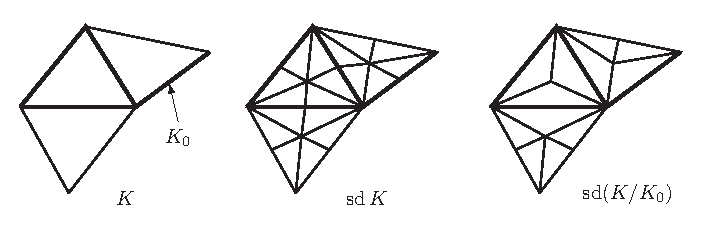
\includegraphics[width=123mm]{figures/2-4-1.pdf}\\图 2.4.1\end{center}
一般单纯逼近定理不能仅靠反复重心剖分证明，因为定理 2.4.2 的 Lebesgue 数论证要求 $|K|$ 紧致。对一般复形，每个单形所需剖分精细程度可能不同，必须允许这种差异。

\entry{定义}{2.4.5}设函数 $N$ 为 $K$ 的每个正维单形 $\sigma$ 指定非负整数 $N(\sigma)$。令 $L_0=K^{(0)}$。设 $L_p$ 为 $p$ 维骨架的剖分，对每个 $(p+1)$ 维单形 $\sigma$，取 $L_p$ 中底空间为 $\Bd\sigma$ 的子复形 $L_\sigma$，先形成锥 $\widehat\sigma*L_\sigma$，再保持 $L_\sigma$ 不变，对此锥作 $N(\sigma)$ 次重心剖分。令 $L_{p+1}$ 为 $L_p$ 与所有
\[
\operatorname{sd}^{N(\sigma)}(\widehat\sigma*L_\sigma/L_\sigma)
\]
的并。于是 $L_{p+1}$ 为 $(p+1)$ 维骨架的剖分，而各 $L_p$ 的并为 $K$ 的剖分，称为\textbf{相应于函数 $N(\sigma)$ 的广义重心剖分}（generalized barycentric subdivision）。

\sourcepage{106}
本节余下部分说明，这种剖分足以证明一般单纯逼近定理。比较下列复形时，可参照图 2.4.1。

\entry{引理}{2.4.6}设 $K_0$ 为 $K$ 的子复形。
\begin{enumerate}[label=(\alph*)]
\item $\operatorname{sd}(K/K_0)$ 的每个单形 $\tau$ 都形如
\[
\tau=\widehat\sigma_1\widehat\sigma_2\cdots\widehat\sigma_q v_0v_1\cdots v_p,
\]
其中 $s=v_0\cdots v_p$ 为 $K_0$ 的单形，各 $\sigma_j$ 是 $K$ 中不属于 $K_0$ 的单形，且 $\sigma_1\succ\cdots\succ\sigma_q\succ s$。
\item 表达式中的 $v_0\cdots v_p$ 或 $\widehat\sigma_1\cdots\widehat\sigma_q$ 可以缺失。$\tau$ 与 $|K_0|$ 不交，当且仅当前一部分缺失；此时 $\tau$ 是 $\operatorname{sd}K$ 的单形。
\end{enumerate}
\noindent\textbf{证明：}(a) 对 $J_0$ 中的单形成立。一般地，若 $\tau\in J_{p+1}\setminus J_p$，则它或者属于 $K_0$，已有所需形式；或者属于某个锥 $\widehat\sigma*J_\sigma$。由归纳假设，$J_\sigma$ 的单形已有所需形式，且其最大面为 $\sigma$ 的真面，添加顶点 $\widehat\sigma$ 后仍是所需形式。

(b) 若后一部分顶点 $v_i$ 存在，则 $\tau$ 至少在 $v_0\cdots v_p$ 上与 $|K_0|$ 相交。反过来，若交非空，则其中包含 $\tau$ 的一个面，因而包含一个顶点。各 $\widehat\sigma_j$ 都不属于 $|K_0|$，故某个 $v_i$ 必须存在。\hfill$\square$

证明一般单纯逼近定理，需要使开星形邻域族加细覆盖
\[
\mathcal A=\{h^{-1}(\operatorname{St}(w,L)):w\text{ 为 }L\text{ 的顶点}\}.
\]
实际上将证明更强的结论：存在剖分 $K'$，使闭星形邻域族 $\{\overline{\operatorname{St}(v,K')}\}$ 加细 $\mathcal A$。下面的引理是归纳步骤的关键。

\sourcepage{107--108}
\entry{引理}{2.4.7}设 $K=p*B$ 为有限复形 $B$ 上的锥，$\mathcal A$ 为 $|K|$ 的开覆盖。假定对 $B$ 的每个顶点 $v$，指定了 $A_v\in\mathcal A$，满足 $\overline{\operatorname{St}(v,B)}\subset A_v$。则存在 $N$，使 $\operatorname{sd}^N(K/B)$ 的闭星形邻域族加细 $\mathcal A$，并且对 $B$ 的每个顶点 $v$，有
\[
\overline{\operatorname{St}(v,\operatorname{sd}^N(K/B))}\subset A_v.
\]
\noindent\textbf{证明：}设 $|B|\subset\R^m\times\{0\}$，$n=\dim K$，取锥顶 $p=(0,\ldots,0,1)\in\R^m\times\R$。

\textbf{第一步。}随着 $N$ 增大，最大单形直径一般不趋于零，因为 $B$ 中的正维面始终不剖分。不过，与平面 $\R^m\times\{0\}$ 相交的单形会越来越贴近该平面。更一般地，设 $K'$ 是保持 $B$ 不变的剖分，且所有与该平面相交的单形都位于条带 $\R^m\times[0,\epsilon]$ 内。则 $\operatorname{sd}(K'/B)$ 中与此平面相交的单形 $\tau$，都位于 $\R^m\times[0,n\epsilon/(n+1)]$ 内。

由引理 2.4.6，$\tau$ 形如 $\widehat\sigma_1\cdots\widehat\sigma_qv_0\cdots v_p$。\translatornote{原文此处误引为引理 2.5.5。}若它与平面相交而不完全位于平面内，则两部分都不缺失，各 $v_i$ 位于平面内。每个 $\sigma_j$ 都以 $v_0\cdots v_p$ 为面，故与平面相交，位于上述条带。设其顶点为 $w_0,\ldots,w_k$，$\pi$ 为最后坐标投影。各 $\pi(w_i)\leq\epsilon$，至少一个为零，因此
\[
\pi(\widehat\sigma_j)=\sum_{i=0}^k\frac1{k+1}\pi(w_i)
\leq\frac k{k+1}\epsilon\leq\frac n{n+1}\epsilon.
\]
$\tau$ 的全部顶点都位于所需凸条带内，故整个单形也位于其中。

\textbf{第二步。}记 $K_N=\operatorname{sd}^N(K/B)$。证明存在 $N_0$，当 $N\geq N_0$ 时，对 $B$ 的每个顶点 $v$，有
\[
\overline{\operatorname{St}(v,K_N)}\subset A_v.\tag{$*$}
\]
先断言，可选择 $\delta>0$，使对每个 $v$，
\[
\overline{\operatorname{St}(v,K)}\cap(\R^m\times[0,\delta])\subset A_v,
\]
见图 2.4.2。
\begin{center}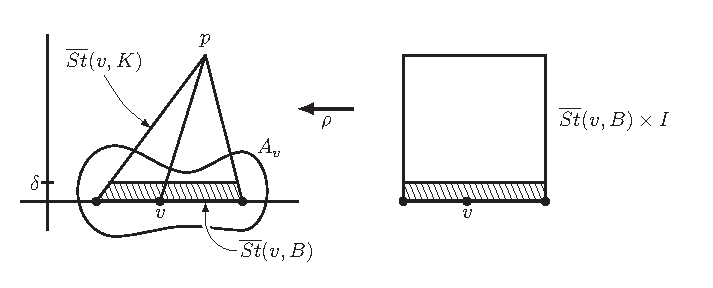
\includegraphics[width=123mm]{figures/2-4-2.pdf}\\图 2.4.2\end{center}
考察连续映射 $\rho:|B|\times I\to|K|$，$\rho(x,t)=(1-t)x+tp$。因为 $K$ 为锥，它把 $\overline{\operatorname{St}(v,B)}\times I$ 映到 $\overline{\operatorname{St}(v,K)}$ 上，并保持最后坐标：
\[
\pi\rho(x,t)=(1-t)\pi(x)+t\pi(p)=(1-t)0+t1=\pi(x,t).
\]
闭星形邻域 $\overline{\operatorname{St}(v,B)}$ 紧致，由一般拓扑的管状引理［例如 [Mun00] 第 26 节］，可选取 $\delta>0$，使
\[
\overline{\operatorname{St}(v,B)}\times[0,\delta]\subset\rho^{-1}(A_v).
\]
更直接地，可用有限多个包含于 $\rho^{-1}(A_v)$ 的集合 $U_i\times[0,\delta_i]$ 覆盖底部，再取 $\delta=\min_i\delta_i$。因为 $B$ 的顶点有限，也可令 $\delta$ 对所有顶点同时适用。于是
\[
\rho(\overline{\operatorname{St}(v,B)}\times[0,\delta])
=\overline{\operatorname{St}(v,K)}\cap(\R^m\times[0,\delta])\subset A_v.
\]
由第一步选择 $N_0$，使 $N\geq N_0$ 时，与底平面相交的各单形都位于此条带。故闭星形邻域 $\overline{\operatorname{St}(v,K_N)}$ 同时位于条带与 $\overline{\operatorname{St}(v,K)}$，所以位于 $A_v$，证明 $(*)$。

\sourcepage{109}
\textbf{第三步。}固定 $N_0$，考察 $K_{N_0+1}$。令 $Q$ 为其中所有与 $B$ 不交的单形的并，见图 2.4.3。用 $P$ 表示图中其余靠近底部的闭区域，即所有与 $B$ 相交的单形之并。\translatornote{原文使用图中的 $P$，但没有在正文中明确给出定义；这里按图及后续论证补明。}
\begin{center}
\begin{minipage}{.47\textwidth}\centering
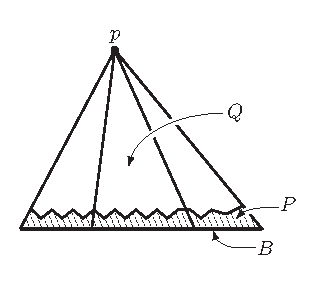
\includegraphics[width=59mm]{figures/2-4-3.pdf}\\图 2.4.3
\end{minipage}\hfill
\begin{minipage}{.47\textwidth}\centering
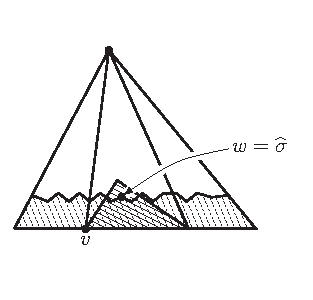
\includegraphics[width=57mm]{figures/2-4-4.pdf}\\图 2.4.4
\end{minipage}
\end{center}
证明：若 $N\geq N_0+1$，$w$ 为 $K_N$ 中位于 $P\setminus|B|$ 的顶点，则存在 $A\in\mathcal A$，使
\[
\overline{\operatorname{St}(w,K_N)}\subset A.\tag{$**$}
\]
先设 $N=N_0+1$。$P$ 按定义是子复形的多胞体。由引理 2.4.6，位于 $P$ 但不在 $B$ 的顶点 $w$ 为某个 $K_{N_0}$ 单形 $\sigma$ 的重心，该 $\sigma$ 与 $B$ 相交而不包含于 $B$，见图 2.4.4。选取其一个位于 $B$ 的顶点 $v$，由引理 2.3.2，
\[
\operatorname{St}(w,K_{N_0+1})\subset\operatorname{St}(v,K_{N_0}).
\]
取闭包，再用第二步，得 $\overline{\operatorname{St}(w,K_{N_0+1})}\subset\overline{\operatorname{St}(v,K_{N_0})}\subset A_v$。

若 $N>N_0+1$，则 $P$ 中的顶点 $w'$ 位于 $K_{N_0+1}$ 的某个顶点 $w$ 的星形邻域内，可取 $w$ 位于 $P$。由引理 2.3.2，$\operatorname{St}(w',K_N)\subset\operatorname{St}(w,K_{N_0+1})$，取闭包后由前段，或 $w\in B$ 时由第二步，得到 $(**)$。

\textbf{第四步。}令 $\lambda$ 为覆盖的 Lebesgue 数。$Q$ 是 $K_{N_0+1}$ 的某个子复形 $J$ 的多胞体。由引理 2.4.6，形成 $K_{N_0+2}$ 时，$J$ 的每个单形都作普通重心剖分，因此 $\operatorname{sd}J$ 为其子复形。重复可知，$\operatorname{sd}^MJ$ 为 $K_{N_0+1+M}$ 的子复形。

选取足够大的 $M$，使 $\operatorname{sd}^MJ$ 的每个单形直径小于 $\lambda/2$。若 $N\geq N_0+1+M$ 且 $w\notin P$，则存在 $A\in\mathcal A$，使
\[
\overline{\operatorname{St}(w,K_N)}\subset A.\tag{$***$}
\]
因为每个以 $w$ 为顶点的单形均位于 $Q$，并包含于上述细剖分的单形中，所以闭星形邻域直径小于 $\lambda$，位于某个覆盖成员中。综合 $(*)$、$(**)$、$(***)$ 即得引理。\hfill$\square$

\sourcepage{110--111}
\entry{定理}{2.4.8}设 $K$ 为复形，$\mathcal A$ 为 $|K|$ 的开覆盖。存在广义重心剖分 $K'$，使其闭星形邻域族加细 $\mathcal A$。

\noindent\textbf{证明：}逐步构造。先令 $L_0=K^{(0)}$，为每个顶点 $v$ 选择包含它的覆盖成员 $A_v$。

一般地，设已给定 $K^{(p)}$ 的剖分 $L_p$，以及为每个顶点 $v$ 指定 $A_v\in\mathcal A$ 的函数 $f_p$，满足 $\overline{\operatorname{St}(v,L_p)}\subset A_v$。下面扩张到 $L_{p+1}$ 及 $f_{p+1}$。

对于每个 $(p+1)$ 维单形 $\sigma$，其边界为 $L_p$ 的某个子复形 $L_\sigma$ 的多胞体。对锥 $\widehat\sigma*L_\sigma$，由引理存在 $N(\sigma)$，使
\[
C(\sigma)=\operatorname{sd}^{N(\sigma)}(\widehat\sigma*L_\sigma/L_\sigma)
\]
满足：若顶点 $v\in L_\sigma$，则 $\overline{\operatorname{St}(v,C(\sigma))}\subset A_v$；对于其他顶点 $w$，存在某个 $A\in\mathcal A$ 包含其闭星形邻域。

令 $L_{p+1}$ 为 $L_p$ 与所有 $C(\sigma)$ 的并。若 $v$ 是旧顶点，则其新闭星形邻域为 $\overline{\operatorname{St}(v,L_p)}$ 与所有包含 $v$ 的相应 $\overline{\operatorname{St}(v,C(\sigma))}$ 的并，全部位于 $A_v$。若 $w$ 为新顶点，则它位于某个 $\sigma$ 的内部，且
\[
\overline{\operatorname{St}(w,L_{p+1})}
=\overline{\operatorname{St}(w,C(\sigma))}.
\]
选取包含它的覆盖成员 $A_w$，定义 $f_{p+1}(w)=A_w$。归纳步骤完成。

取 $K'=\bigcup_p L_p$，函数 $f$ 为各 $f_p$ 的并。若 $v$ 是 $L_p$ 的顶点，则对所有 $k\geq0$，有 $\overline{\operatorname{St}(v,L_{p+k})}\subset f_{p+k}(v)=f(v)=A_v$。因此 $\overline{\operatorname{St}(v,K')}\subset A_v$，定理得证。\hfill$\square$

\entry{定理}{2.4.9（一般单纯逼近定理）}设 $K,L$ 为复形，$h:|K|\to|L|$ 连续。存在 $K$ 的剖分 $K'$，使 $h$ 有单纯逼近 $f:K'\to L$。

\noindent\textbf{证明：}用开集 $h^{-1}(\operatorname{St}(w,L))$ 覆盖 $|K|$，选择闭星形邻域族加细此覆盖的剖分 $K'$。于是 $h$ 对 $K',L$ 满足星形条件。\hfill$\square$

\subsection*{习题}
\begin{enumerate}
\item \begin{enumerate}[label=(\alph*)]
\item 用定理 2.4.2 证明：若 $K,L$ 有限，$\dim K=m$，则每个连续映射 $h:|K|\to|L|$ 同伦于将 $K$ 映入 $L^{(m)}$ 的映射。［提示：第 2.2 节习题 2。非有限情形后面讨论。］
\item 证明：若 $h:S^m\to S^n$ 且 $m<n$，则 $h$ 同伦于常值映射。［提示：任意 $f:X\to S^n\setminus\{p\}$ 同伦于常值映射。］
\end{enumerate}
\item 若 $h:|K|\to|L|$ 连续，给定 $\epsilon>0$，证明存在两者的剖分 $K',L'$ 以及单纯映射 $f:K'\to L'$，使对所有 $x$ 有 $|f(x)-h(x)|<\epsilon$。
\item 证明：若 $\dim K=m$，则 $|K|$ 的覆盖维数至多为 $m$，见第 2.3 节习题。
\item 举例说明习题 3 的结论是最佳的。
\end{enumerate}
